\section{Subjetivismo}
Es la teoría de valor de acuerdo a lo subjetivo, el comunista piensa que el valor de los bienes son objetivos, un comunista pretende planear todo desde arriba. \newline 
Valor de los bienes es subjetivo, bienes tienen función de acurdo necesidades que satisfacen, tiene valor para alguien y para otra persona pueda que no tenga valor. Si la teoría del valor fuese cierta ninguna empresa quebraría. Si la cantidad de trabajo determina el precio simplemente cualquiera quisiera meterle hasta trabajo de por gusto. \newline 
Teoría de subjetivismo: el valor se determina por qué tan bien satisfacen las necesidades existentes.

\section{Marginalismo}
El marginalismo, la paradoja de el agua y los diamantes, las necesidades o el valor de los bienes viene dado de la necesidad marginal, el ultimo de los fines que permite conseguir, toda decisión se toma al margen. El valor que tiene la unidad, la ultima unidad de algún bien.

\begin{center}
    \begin{figure}[htbp]
        \centering
        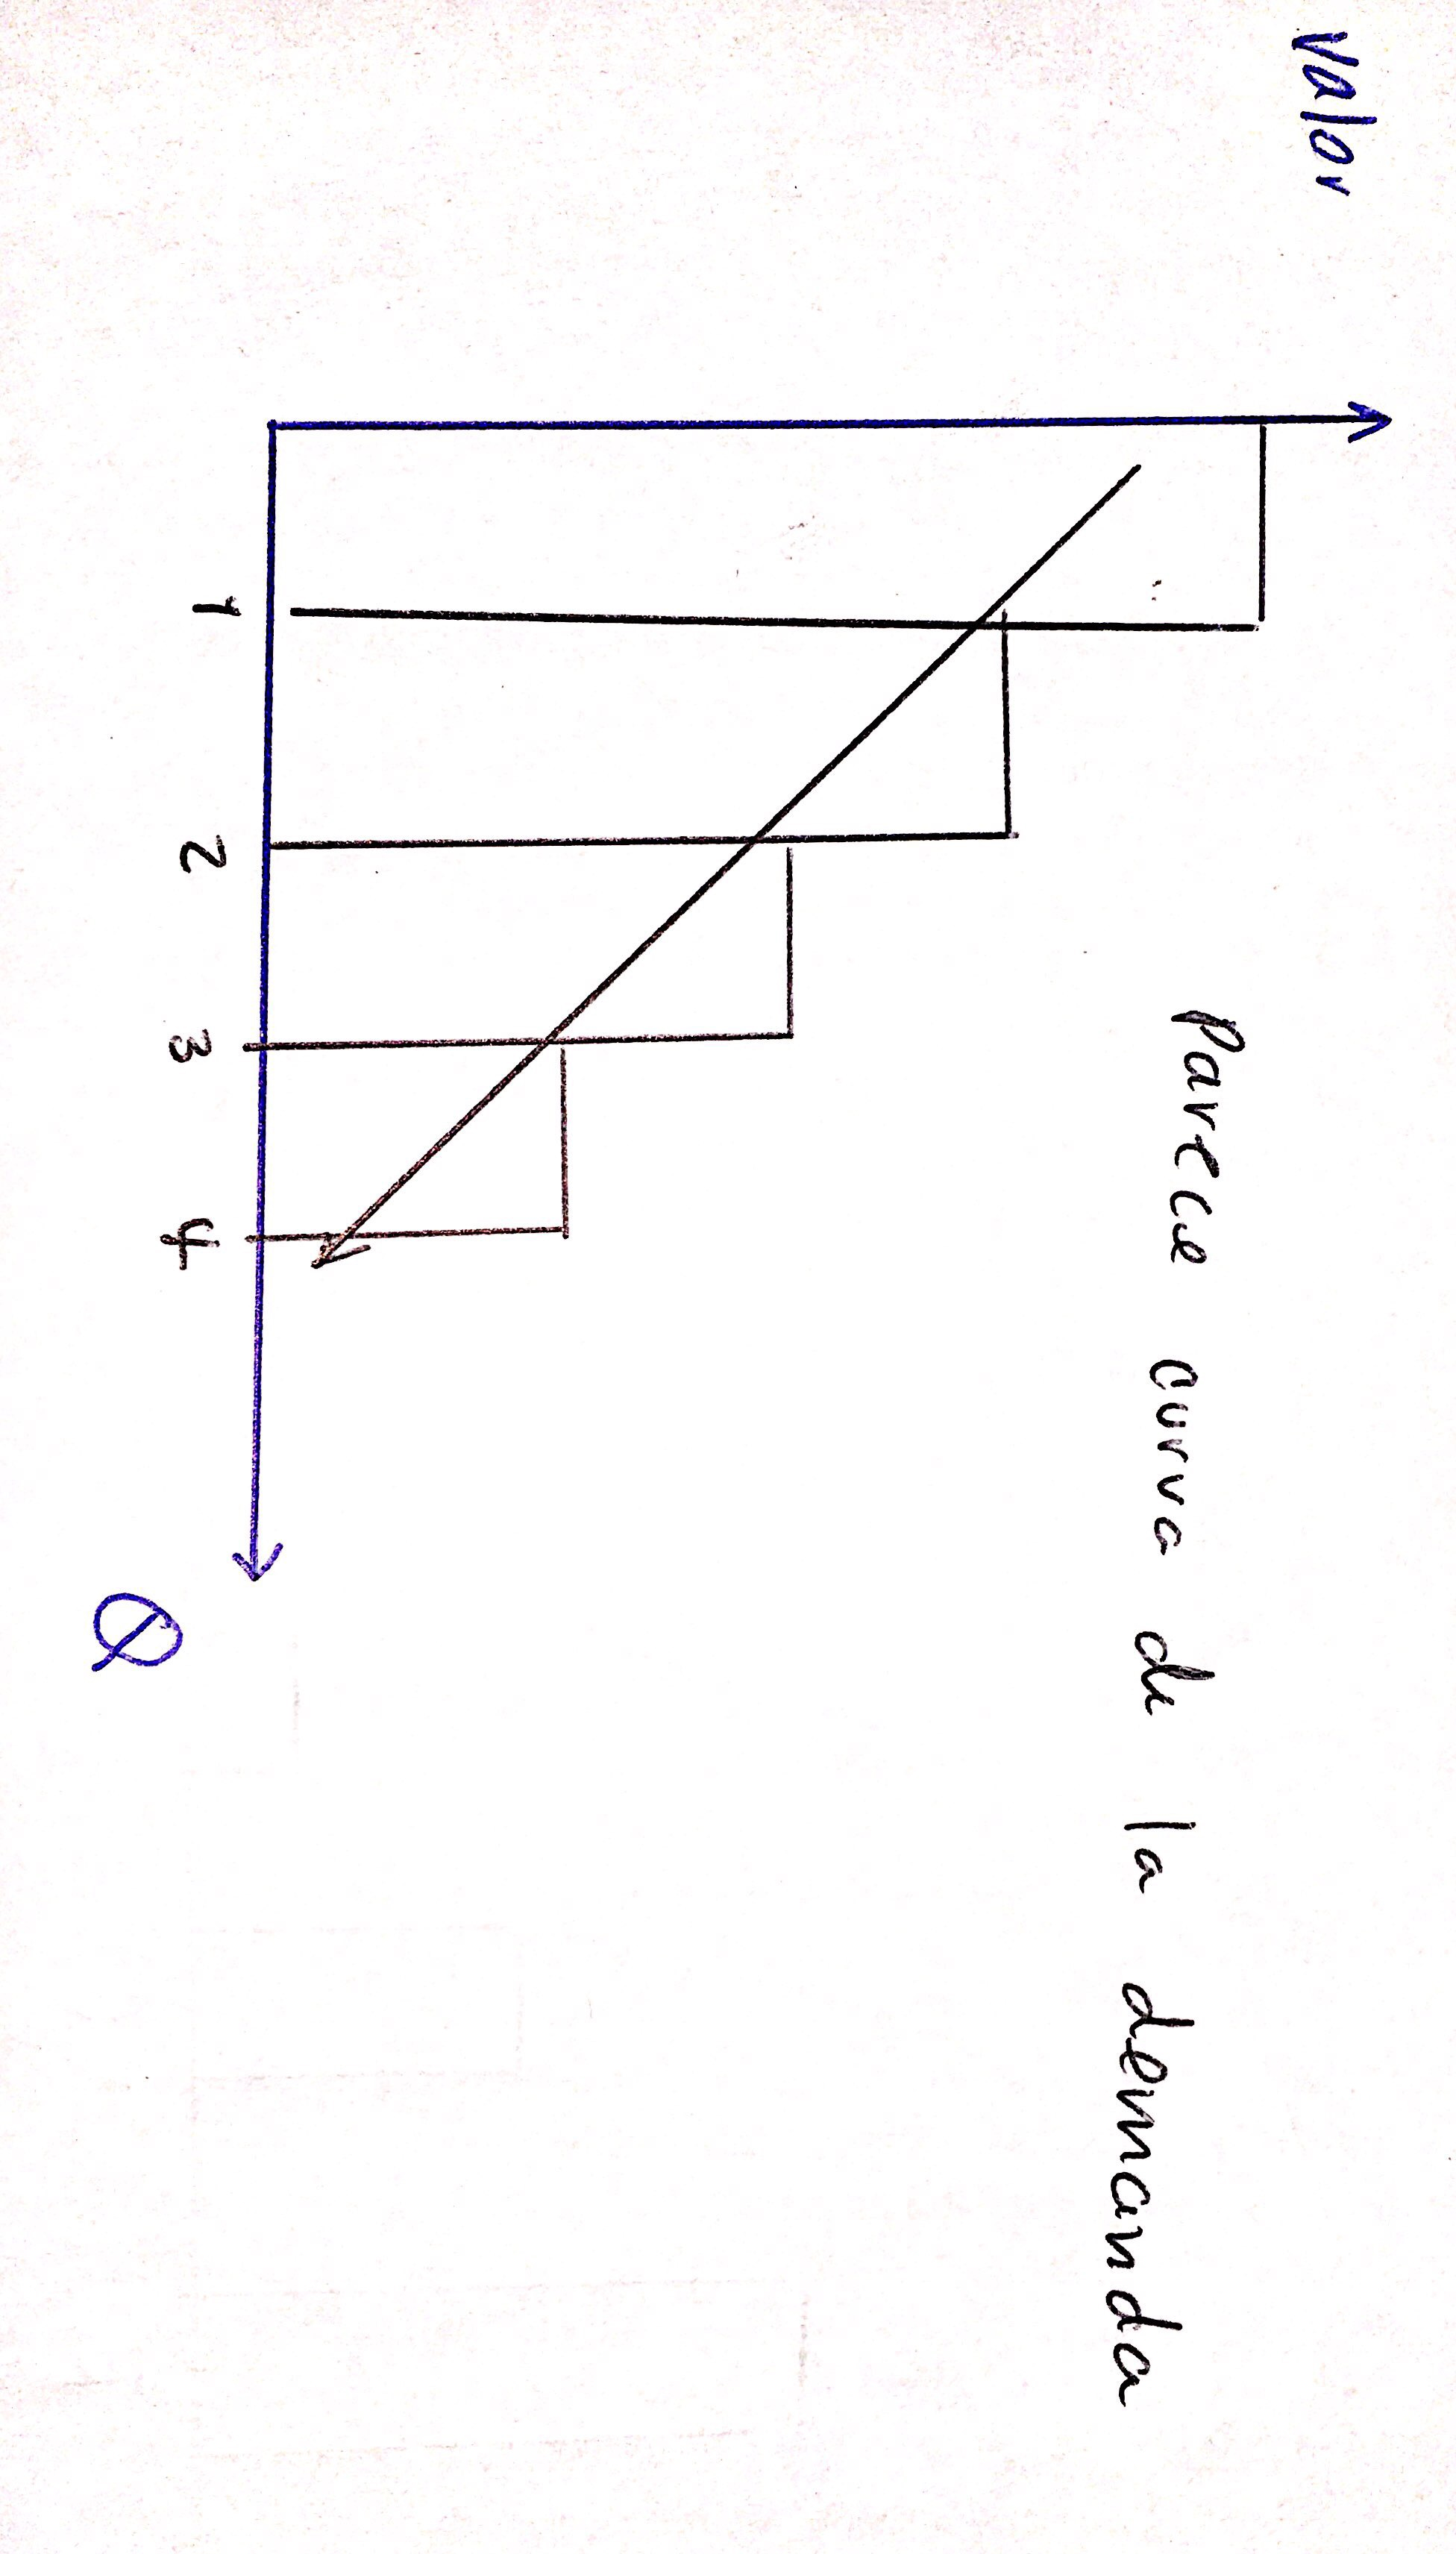
\includegraphics[width=6cm,angle=90]{Classes/Images/2019-07-24-1.jpg}
        \caption{La marginalidad tambien se puede representar como una curva de demanda también}
        \label{fig1}
    \end{figure}
\end{center}

% \vspace{10pt}
\begin{center}
    \begin{figure}[htbp]
        \centering
        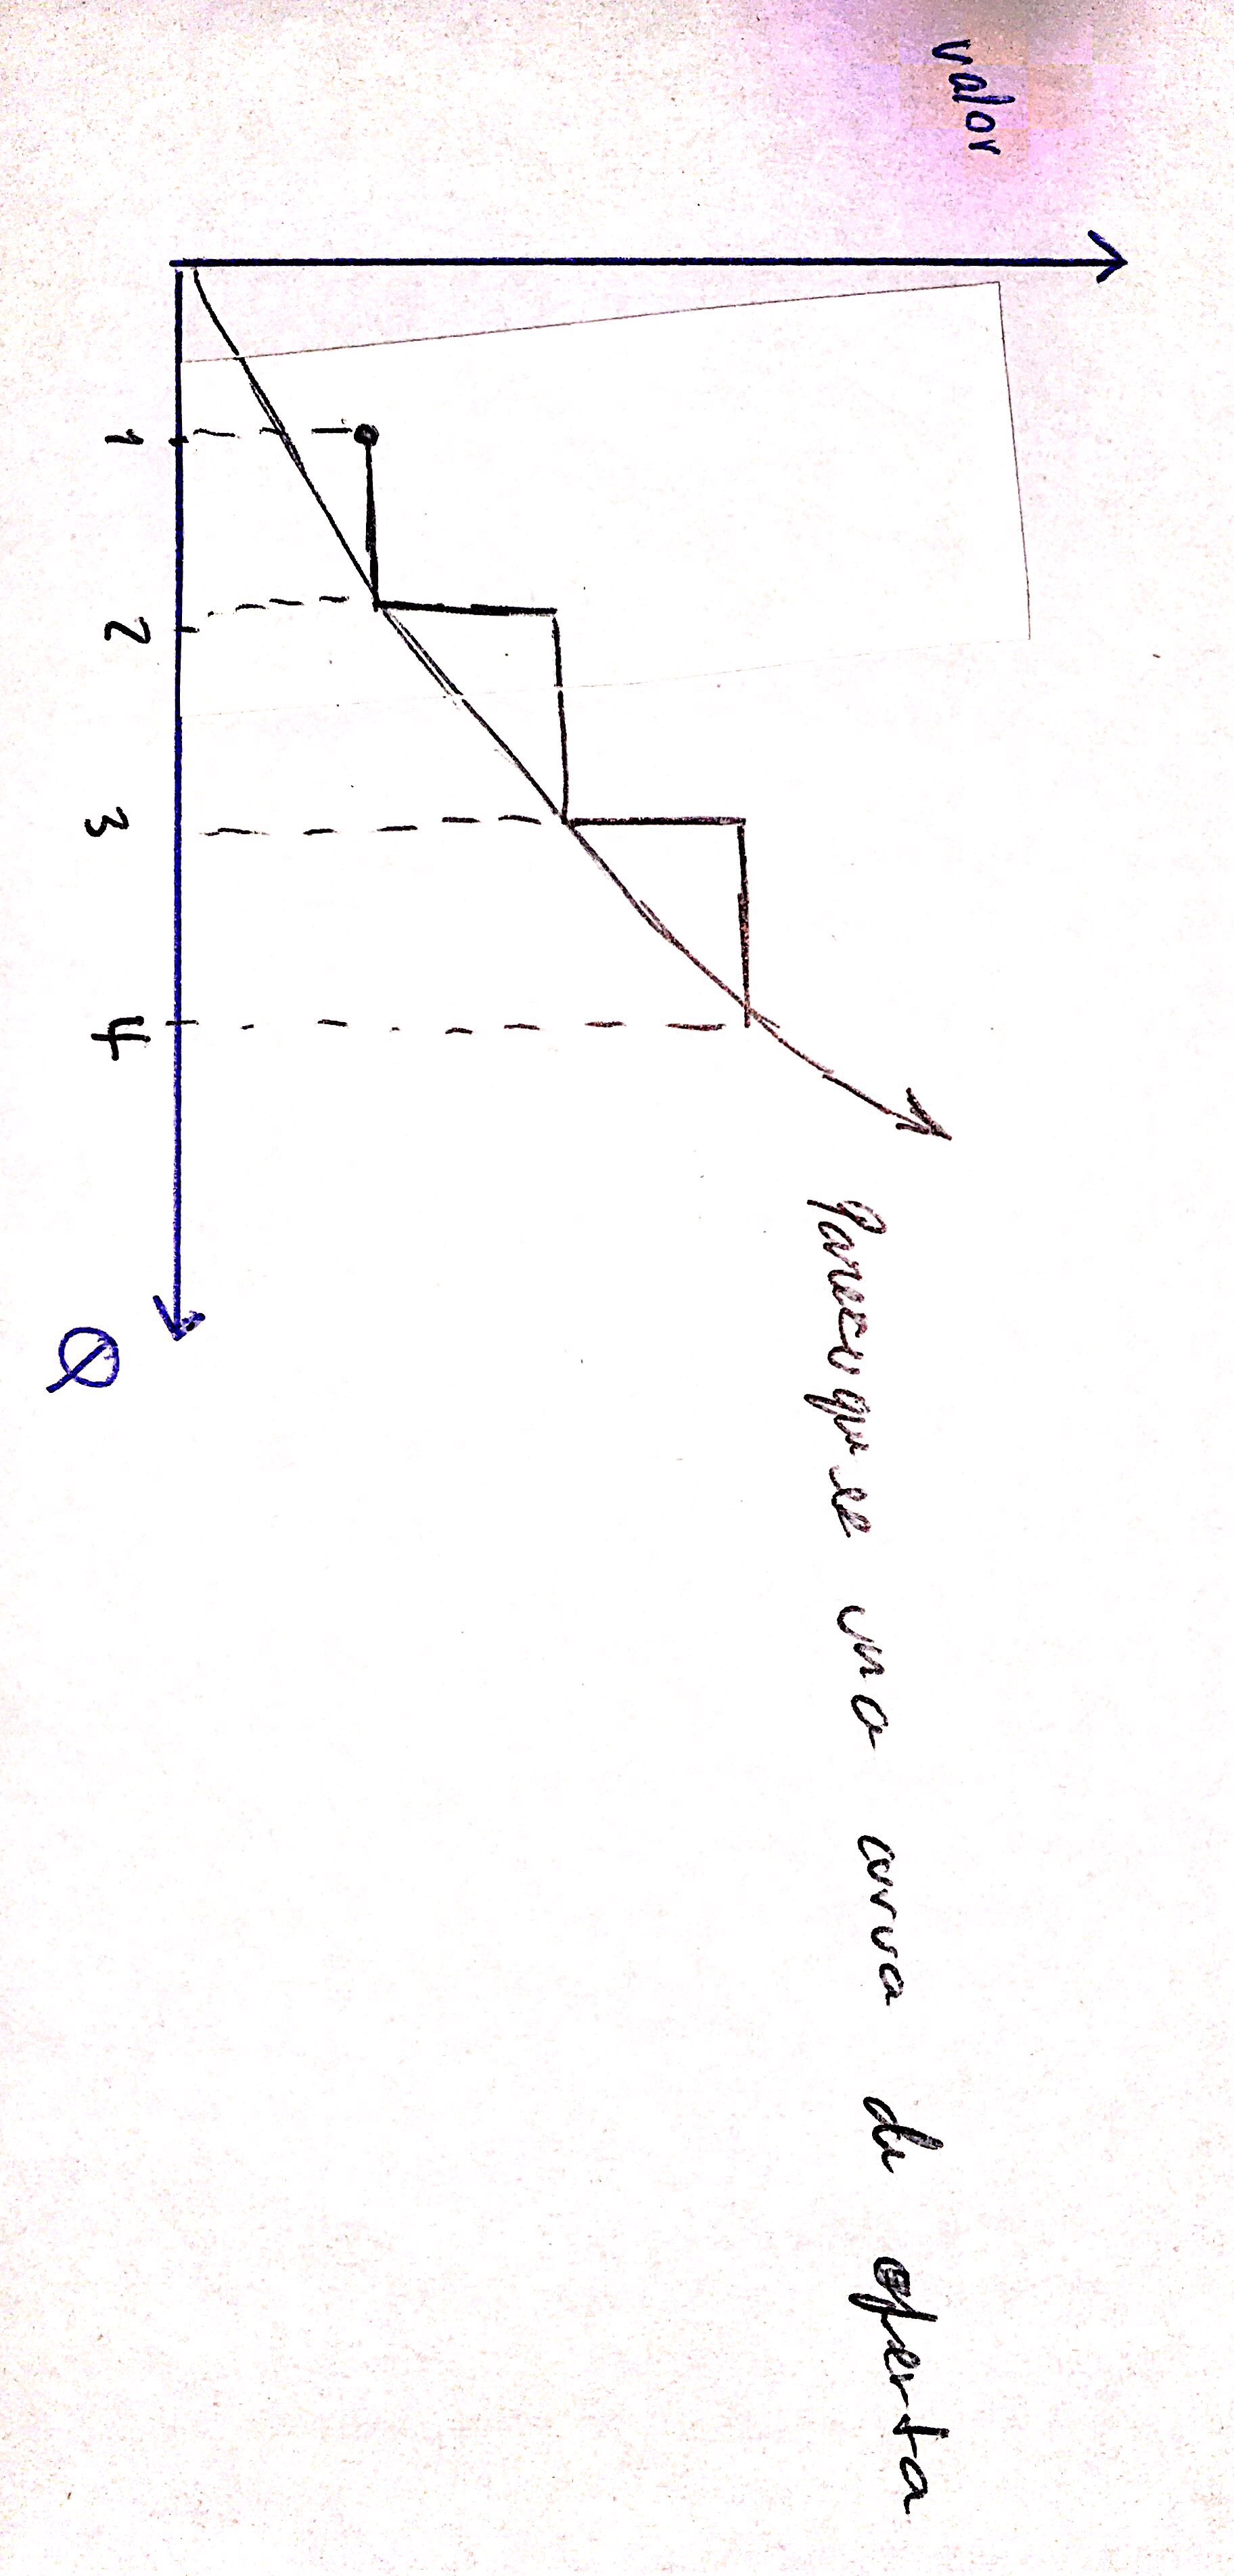
\includegraphics[width=6cm,angle=90]{Classes/Images/2019-07-24-2.jpg}
        \caption{La marginalidad puede interpretarse como una curva de oferta tembién}
        \label{fig2}
    \end{figure}
\end{center}




\section{Oferta y demanda}
Teoría de la utilidad marignal, el principio de utilidad marginal decreciente es \textbf{siempre} decreciente. El reverso de la teoría marginal decreciente coste marginal creciente; la utilida de una unidad más conlleva que todas las unidades van a disminuir de valor.
\begin{center}
    \begin{figure}[htbp]
        \centering
        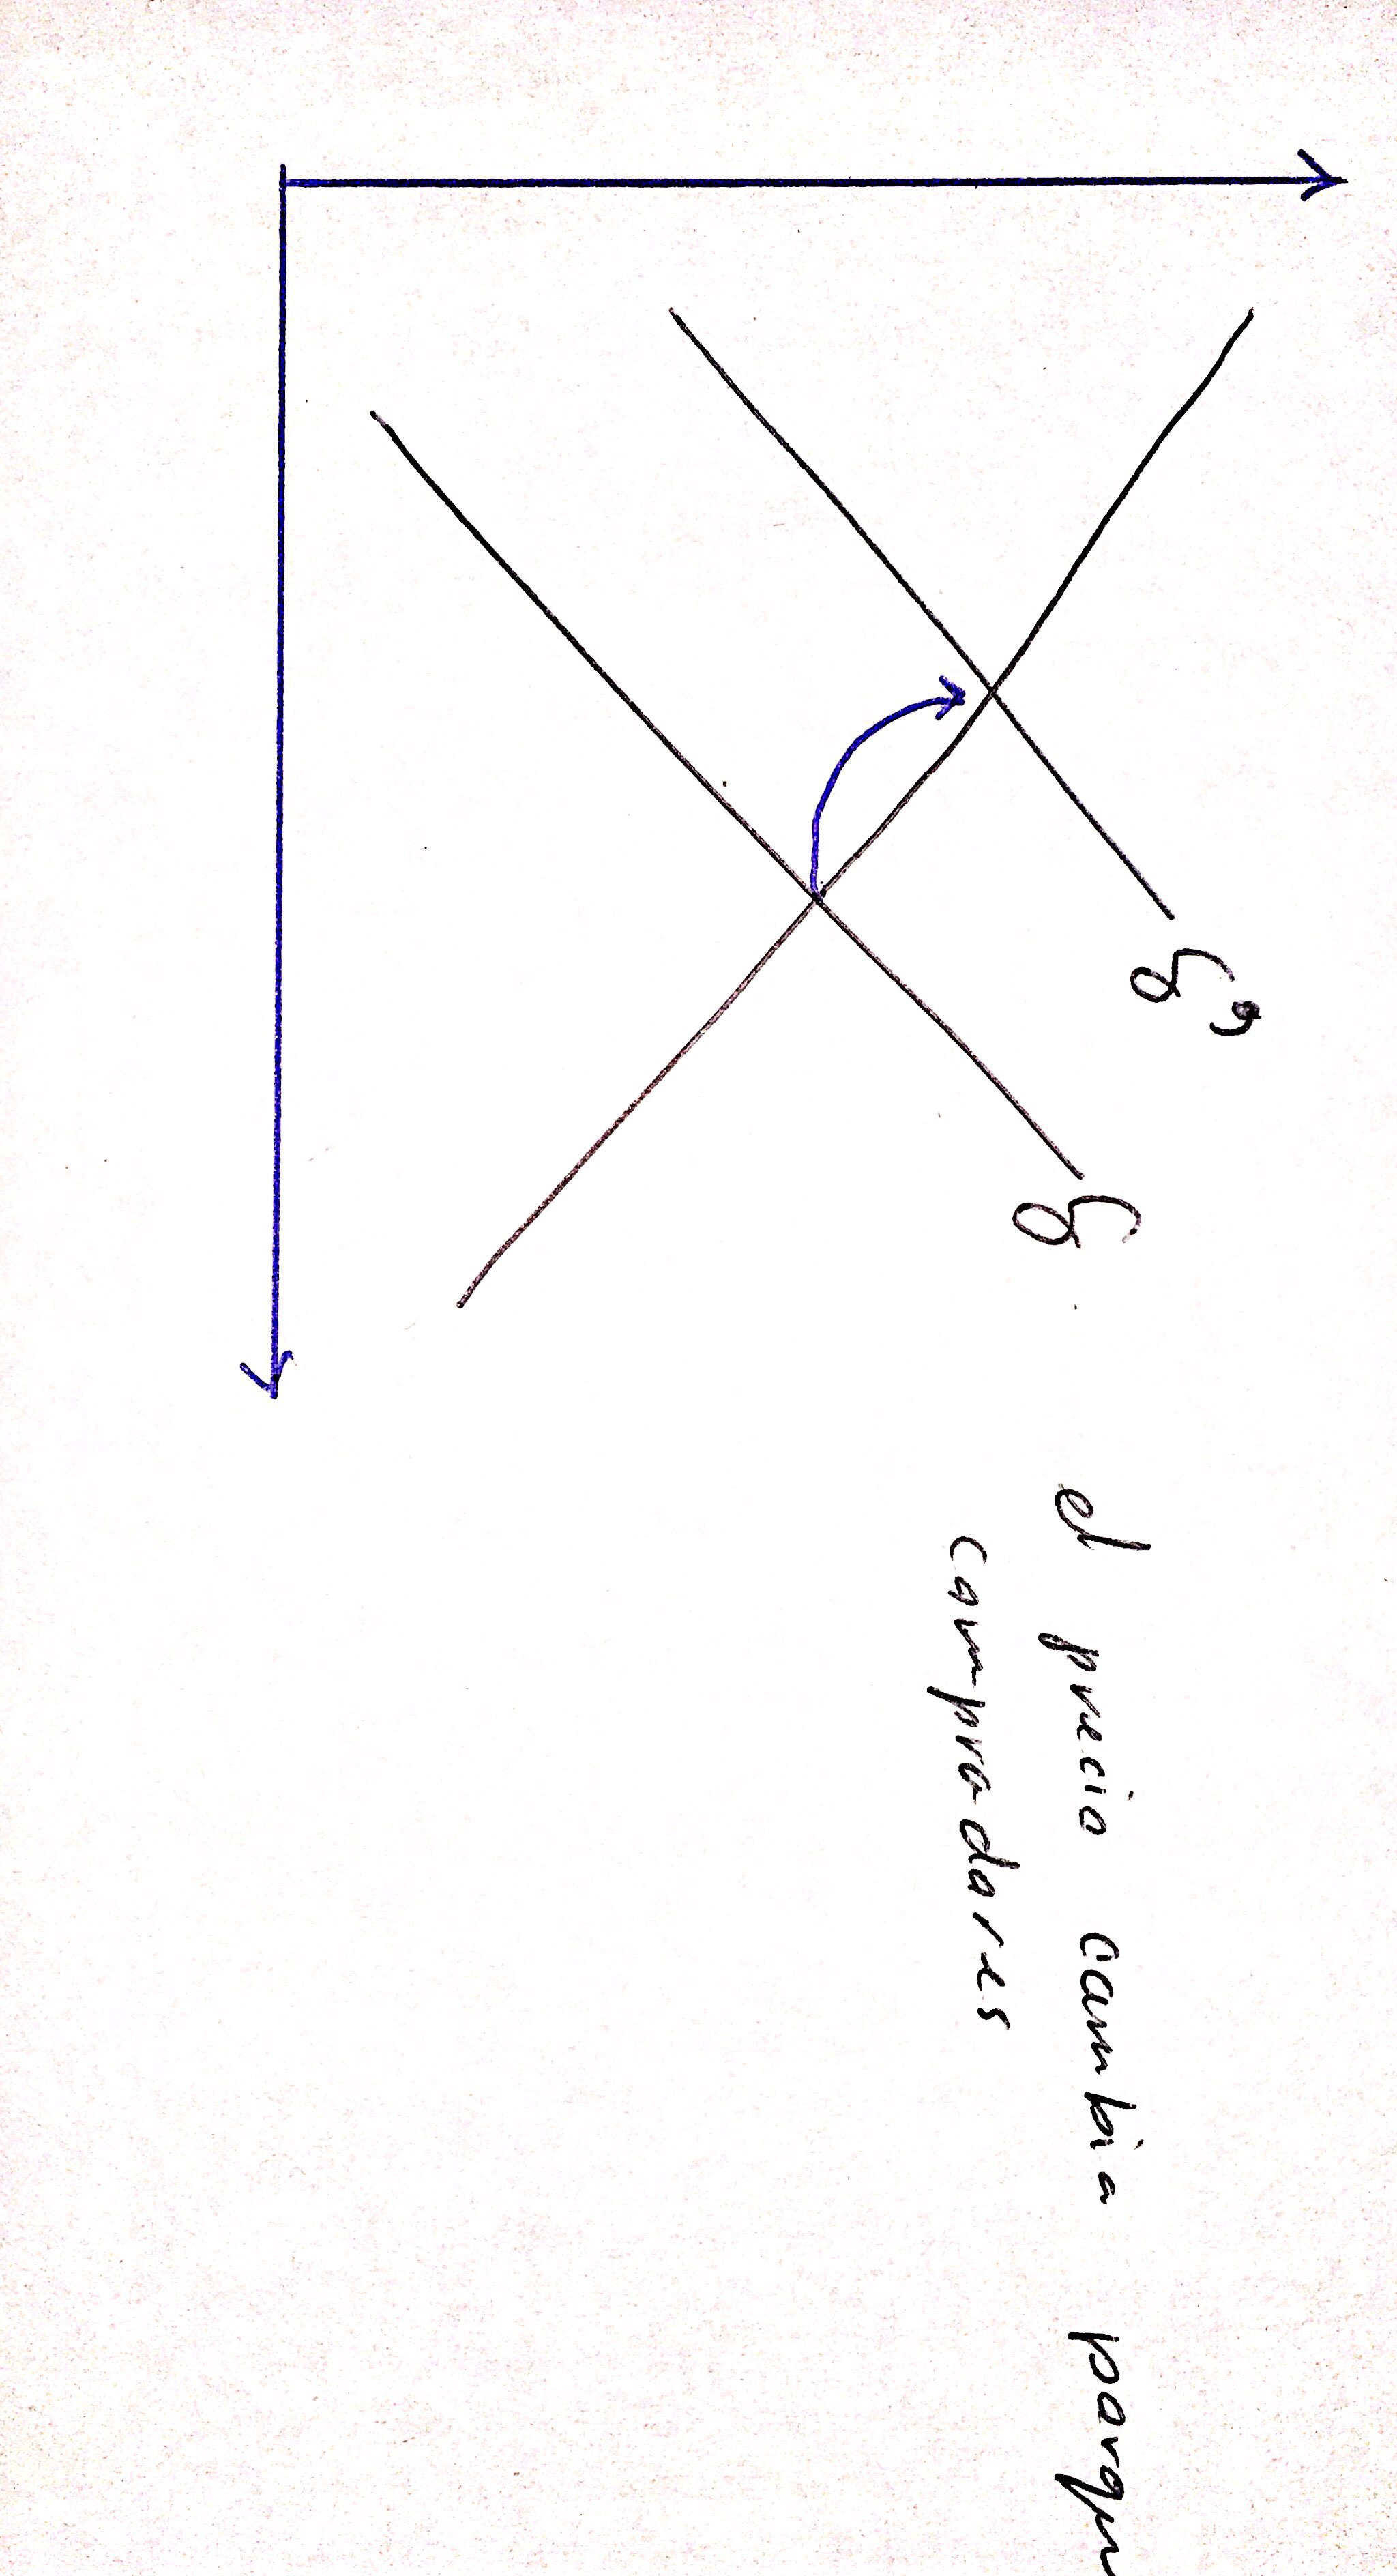
\includegraphics[width=6cm,angle=90]{Classes/Images/2019-07-24-3.jpg}
        \caption{El precio cambia porque los compradores designan una utilidad diferente cada vez y es subjetiva, al igual que los oferentes}
        \label{fig3}
    \end{figure}
\end{center}


\section{Sistema de precios}
Informa de manera indirecta, sobre que producir, con quién producirlo, cuánto producirlo y para quién producirlo. \textbf{Nos preguntamos:} ¿el precio es el determinante o el determinado? El sistema de precio es el determinado. Ejemplo, si un precio sube alguien va a tender a querer meterse a producirlo. El sistema de precios comunica información esencial para que las personas puedan actuar. Es una dinamica de precios que previene la escasez. En general los empresarios persiguen beneficios altos, por eso un empresario le puede parecer mas rentable producir mesas que producir iPhones. Tasa de rentabilidad, qué tanto te vas a tardar en recuperar la inversión. \newline 
Las rentabilidades altas se detruyen con competencia, se tiende a equilibrar, termino 12.27.
% insertar graficas aqui rentabilida.
\begin{center}
\begin{figure}[htbp]
    \centering
    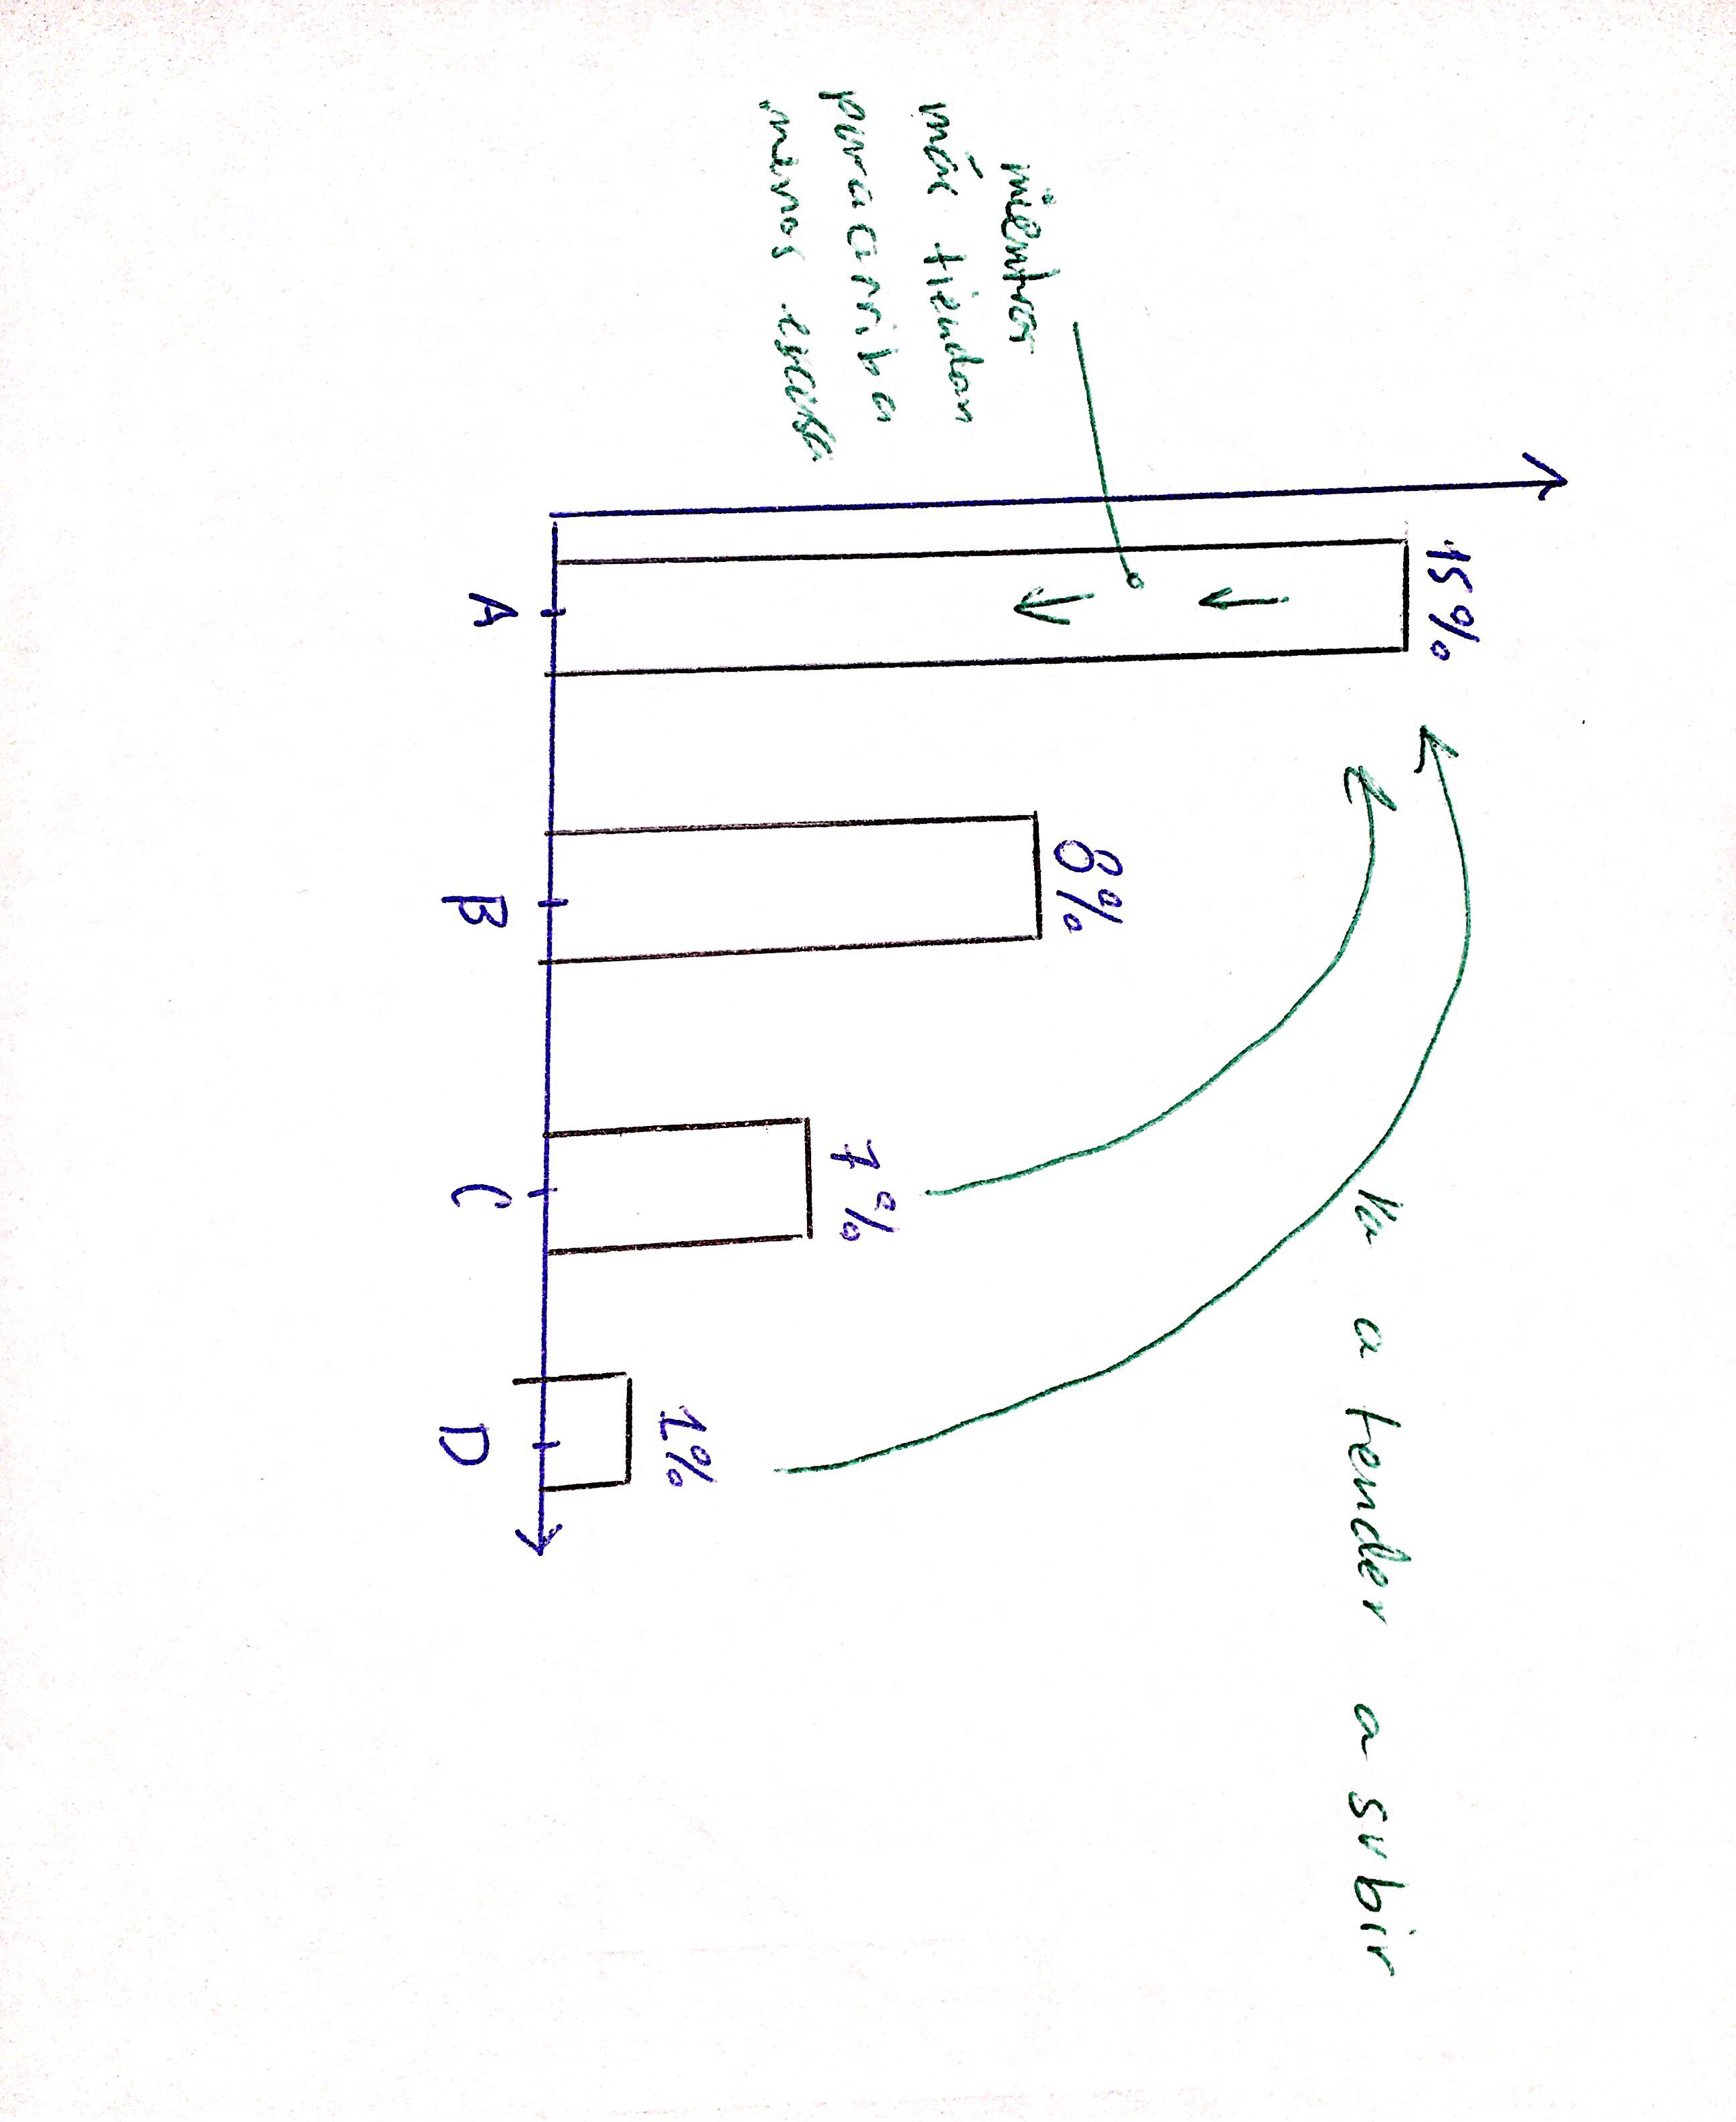
\includegraphics[width=8cm,angle=90]{Classes/Images/2019-07-24-4.jpg}
    \caption{Tiende al equilibrio}
    \label{fig4}
\end{figure}
\end{center}


\section{Subcidios e impuestos}
Si quieres más de algo lo subsidias, si quieres menos de algo pones impuestos. \textbf{Ejemplo: } los ecofiltros regalados, los usaban para masetas, se sobre utiliza. \newline 
\textbf{Ejemplo: } Impuesto a gasolina, se hace caro y la gente lo consume menos. 

\section{Fijación de precios}
Cuando ponen un precio tope se producen faltantes, \textbf{Ejemplo: } el precio de arroz es 3, se presume que es para que toda la gente lo pueda comprar, pero se produce información distorsionada en el sistema de precios y la gente lo empieza a ya no valorarlo. \textbf{Ejemplo: } Venezuela, se controla el harina y el pan, lo que termina produciendo es que todas las panaderías están vacías, si se ponen precios topes se agotan en seguida y nadie le sale rentable producir entonces no se produce. \textbf{Ejemplo: } Los taxis, están a punto de ser erradicado, hay precio minimo de 25Q y ahora lo que ocurre es que los taxis ya no se usan, el precio tope busca controlar la oferta. \textbf{Ejemplo: } El salario mínimo, mientras más pujan el precio del salario minimo para arriba, se aumenta la demanda y se disminuye la oferta, todas las cosas como seguro social, aguinaldo, bono 14, y el salario mínimo termina siendo carísimo. 

\section{Noticia}
Quiz el lunes de la lectura, resumir y analizar la noticia en 5 minutos. 

